\documentclass[aspectratio=169, 10pt]{beamer}

% --- PACKAGES ---
\usepackage[utf8]{inputenc}
\usepackage{tikz}
\usetikzlibrary{shapes.geometric, arrows.meta, positioning, fit, backgrounds, calc}
\usepackage{booktabs}
\usepackage{array}
\usepackage{xcolor}

% --- COLOR PALETTE (flat, white background, single accent) ---
\definecolor{Ink}{HTML}{1A1D23}
\definecolor{Dim}{HTML}{6B7280}
\definecolor{Accent}{HTML}{2C5F8A}
\definecolor{AccentSoft}{HTML}{EFF3F7}
\definecolor{Line}{HTML}{D8DCE2}
\definecolor{Warn}{HTML}{9A4B3C}

% --- BEAMER THEME CUSTOMIZATION ---
\setbeamercolor{background canvas}{bg=white}
\setbeamercolor{normal text}{fg=Ink}
\setbeamercolor{title}{fg=Ink}
\setbeamercolor{subtitle}{fg=Dim}
\setbeamercolor{author}{fg=Dim}
\setbeamercolor{date}{fg=Dim}
\setbeamercolor{item}{fg=Accent}
\setbeamercolor{subitem}{fg=Dim}
\setbeamercolor{block title}{bg=AccentSoft, fg=Accent}
\setbeamercolor{block body}{bg=white, fg=Ink}
\setbeamertemplate{itemize items}[circle]
\setbeamertemplate{navigation symbols}{}
\setbeamertemplate{blocks}[rounded][shadow=false]
\setlength{\parskip}{0pt}

\setbeamertemplate{frametitle}{
  \vspace{0.25cm}
  {\large\bfseries\color{Ink}\insertframetitle}\\[1pt]
  {\footnotesize\color{Dim}\insertframesubtitle}\\[3pt]
  \color{Line}\rule{\linewidth}{0.6pt}\\[4pt]
}
\setbeamertemplate{footline}{
  \hfill\raisebox{6pt}{\color{Dim}\scriptsize\insertframenumber\,/\,\inserttotalframenumber}\hspace{8pt}\vspace{2pt}
}
\setbeamertemplate{title page}{
  \vspace{2.2cm}
  {\color{Line}\rule{\linewidth}{0.6pt}}\\[0.5cm]
  {\centering\Huge\bfseries\color{Ink}\inserttitle\par}
  \vspace{0.25cm}
  {\centering\large\color{Accent}\insertsubtitle\par}
  \vspace{0.6cm}
  {\centering\normalsize\color{Dim}\insertauthor\par}
  \vspace{0.15cm}
  {\centering\normalsize\color{Dim}\insertdate\par}
  \vspace{0.4cm}
  {\color{Line}\rule{\linewidth}{0.6pt}}
}

% --- METADATA ---
\title{VANGUARD-32}
\subtitle{Autonomous Smart Perimeter Defense \& Active Countermeasure Platform}
\author{ATmega32-Based Embedded Systems Design}
\date{Project Proposal}

\begin{document}

% --- SLIDE 1: TITLE ---
\begin{frame}
    \titlepage
\end{frame}

% --- SLIDE 2: MOTIVATION - PROBLEM DESCRIPTION & IMPORTANCE ---
\begin{frame}{1. Motivation}{Problem Description \& Importance}
    \begin{columns}[T]
        \begin{column}{0.48\textwidth}
            \begin{block}{Problem Description}
                \small
                \begin{itemize}
                    \item Conventional installations rely on a single sensor trigger (PIR, optic tripwire).
                    \item False alarms from wind, foliage, and small animals; no automated local verification.
                    \item Passive design: sensors cannot re-orient toward an intrusion sector or discriminate personnel from intruders.
                \end{itemize}
            \end{block}
        \end{column}
        \begin{column}{0.48\textwidth}
            \begin{block}{Why It Matters}
                \small
                \begin{itemize}
                    \item Critical infrastructure, remote outposts, and industrial zones need target acquisition and verification without human latency.
                    \item Reducing false alarms while keeping detection reliability is a core embedded-defense challenge.
                    \item A multi-stage verification pipeline is required before an alarm or countermeasure fires.
                \end{itemize}
            \end{block}
        \end{column}
    \end{columns}
\end{frame}

% --- SLIDE 3: MOTIVATION - WHY THIS PROJECT & OBJECTIVES ---
\begin{frame}{1. Motivation}{Why This Project \& Main Objectives}
    \small The project integrates multi-sensor fusion, closed-loop actuation, multi-bus digital communication, and low-latency interrupt handling on a resource-constrained 8-bit MCU (ATmega32) -- a complete embedded system, not an isolated sensor demo.
    \vspace{0.2cm}
    \begin{enumerate}
        \small
        \item \textbf{Multi-sector triangulation:} 180$^\circ$ field split into 3 sectors, hardware interrupts.
        \item \textbf{Pan-tilt acquisition:} 2-axis turret aligns to the target vector within 500 ms via hardware PWM.
        \item \textbf{Multi-modal verification:} thermal $\Delta T$ (MLX90614) and ToF distance $R$ (VL53L0X) over I$^2$C.
        \item \textbf{Wireless IFF handshake:} encrypted RF badge authentication over SPI to prevent friendly engagement.
        \item \textbf{Active countermeasure:} strobe pulse / solenoid actuation on confirmed hostile target.
        \item \textbf{Telemetry \& black-box logging:} live radar view over UART; on-board MicroSD incident log.
    \end{enumerate}
\end{frame}

% --- SLIDE 4: EQUIPMENT - HARDWARE ---
\begin{frame}{2. Equipment}{Hardware Components}
    \footnotesize
    \begin{columns}[T]
        \begin{column}{0.5\textwidth}
            \begin{itemize}
                \item \textbf{ATmega32-16PU} -- system controller
                \item \textbf{RCWL-0516 / PIR array} -- sector detection (INT0/1/2)
                \item \textbf{MLX90614} -- IR thermal sensor (I$^2$C)
                \item \textbf{VL53L0X} -- laser ToF distance (I$^2$C)
                \item \textbf{nRF24L01+ ($\times$2)} -- 2.4 GHz IFF link (SPI)
            \end{itemize}
        \end{column}
        \begin{column}{0.5\textwidth}
            \begin{itemize}
                \item \textbf{MicroSD module} -- black-box logging (SPI)
                \item \textbf{SG90 / MG996R servos ($\times$2)} -- pan-tilt turret (PWM)
                \item \textbf{FT232RL} -- USB-UART telemetry bridge, 115200 baud
                \item \textbf{MOSFET drivers + solenoid/strobe} -- countermeasure output
                \item \textbf{16$\times$2 I$^2$C LCD} + \textbf{LM2596 buck converters ($\times$2)}
            \end{itemize}
        \end{column}
    \end{columns}
\end{frame}

% --- SLIDE 5: EQUIPMENT - RATIONALE ---
\begin{frame}{2. Equipment}{Why These Components}
    \scriptsize
    \begin{columns}[T]
        \begin{column}{0.48\textwidth}
            \begin{block}{Sensing \& Detection}
                \begin{itemize}
                    \item \textbf{ATmega32:} on-chip TWI, SPI, USART, and two 8-bit timers cover every required bus and PWM channel without external bridge chips.
                    \item \textbf{RCWL-0516/PIR:} outputs a digital edge directly on an interrupt pin -- sub-ms detection with zero MCU polling.
                    \item \textbf{MLX90614:} factory-calibrated digital I$^2$C output (addr.\ 0x5A) -- no analog front end or ADC channel needed.
                    \item \textbf{VL53L0X:} laser ToF gives direct mm-accurate range (addr.\ 0x29) on the same I$^2$C bus, avoiding ultrasonic beam-spread error.
                \end{itemize}
            \end{block}
        \end{column}
        \begin{column}{0.48\textwidth}
            \begin{block}{Actuation, Comms \& Power}
                \begin{itemize}
                    \item \textbf{Servos:} accept a standard 50 Hz PWM signal directly from Timer0/Timer2 OC pins -- no motor driver IC required.
                    \item \textbf{nRF24L01+ / MicroSD:} both are SPI slaves, sharing one hardware bus via independent chip-select lines instead of two controllers.
                    \item \textbf{FT232RL:} the ATmega32 has no native USB peripheral; this bridges USART to a PC USB port.
                    \item \textbf{MOSFET + solenoid/strobe:} MCU I/O pins cannot source actuator current; the MOSFET is a low-side switch driven by one GPIO.
                    \item \textbf{Dual LM2596 rails:} isolates noisy servo current draw from the logic supply, preventing brown-out resets.
                \end{itemize}
            \end{block}
        \end{column}
    \end{columns}
\end{frame}

% --- SLIDE 6: EQUIPMENT - SOFTWARE ---
\begin{frame}{2. Equipment}{Software \& Development Tools}
    \begin{columns}[T]
        \begin{column}{0.5\textwidth}
            \begin{block}{Toolchain}
                \small
                \begin{itemize}
                    \item \textbf{Microchip Studio / AVR-GCC} -- C development, register-level drivers, compilation
                    \item \textbf{USBasp / eXtreme Burner} -- firmware flashing
                    \item \textbf{Proteus VSM} -- circuit simulation before fabrication
                \end{itemize}
            \end{block}
        \end{column}
        \begin{column}{0.5\textwidth}
            \begin{block}{Host-Side Tools}
                \small
                \begin{itemize}
                    \item \textbf{Python 3 (PySerial)} -- UART telemetry parsing
                    \item \textbf{Pygame / Tkinter} -- real-time PC tactical radar GUI
                \end{itemize}
            \end{block}
        \end{column}
    \end{columns}
    \vspace{0.2cm}
    \footnotesize\color{Dim} Sensors provide raw data; the ATmega32 fuses it and drives the response; host tools give visibility only -- the MCU operates autonomously without the PC link.
\end{frame}

% --- SLIDE 7: SYSTEM DESIGN - BLOCK DIAGRAM (redesigned) ---
\begin{frame}{3. System Design}{Block Diagram}
    \centering
    \resizebox{0.93\textwidth}{!}{
        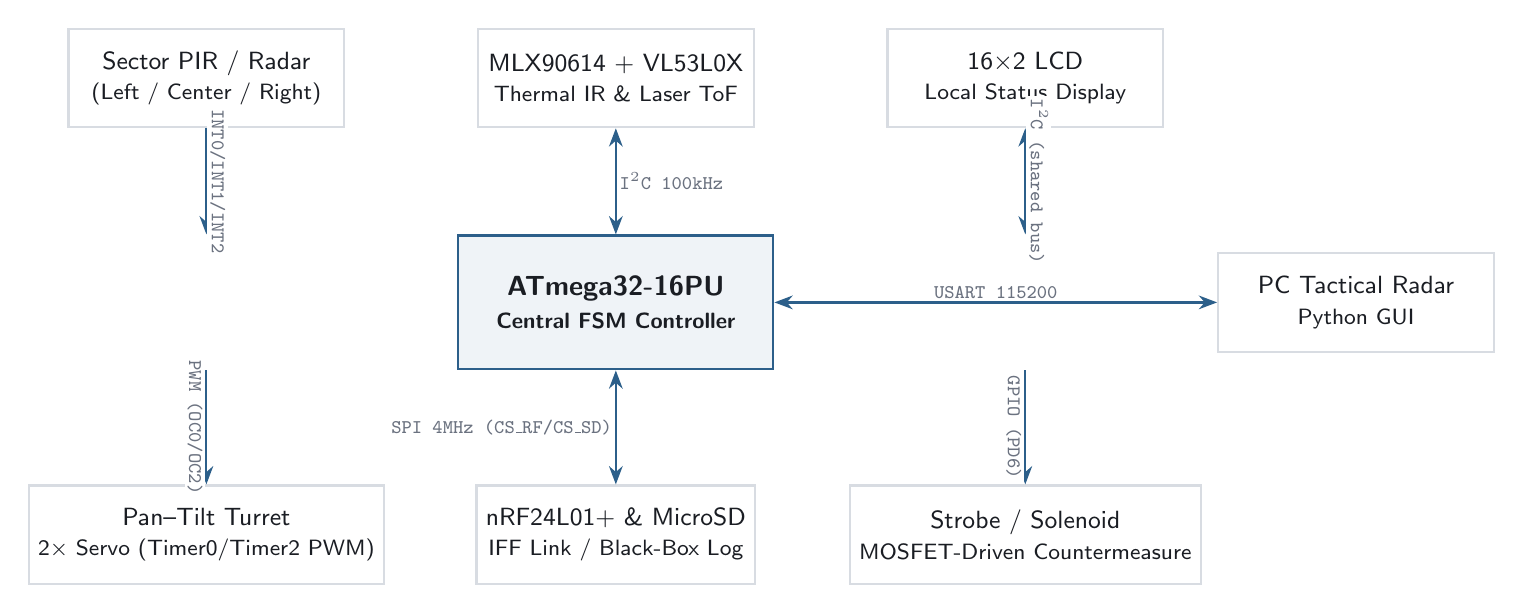
\begin{tikzpicture}[
            mcu/.style={rectangle, draw=Accent, thick, fill=AccentSoft, minimum height=1.7cm, minimum width=4cm, align=center, font=\sffamily\bfseries\normalsize, text=Ink},
            block/.style={rectangle, draw=Line, thick, fill=white, minimum height=1.25cm, minimum width=3.5cm, align=center, font=\sffamily\small, text=Ink},
            arrow/.style={-Stealth, thick, color=Accent},
            biarrow/.style={Stealth-Stealth, thick, color=Accent},
            lbl/.style={font=\scriptsize\ttfamily, color=Dim, fill=white, inner sep=1pt}
        ]
            % Sensing layer (top)
            \node[block] (pir) at (-5.2,3.0) {Sector PIR / Radar\\\footnotesize (Left / Center / Right)};
            \node[block] (thermtof) at (0,3.0) {MLX90614 + VL53L0X\\\footnotesize Thermal IR \& Laser ToF};
            \node[block] (lcd) at (5.2,3.0) {16$\times$2 LCD\\\footnotesize Local Status Display};

            % Central controller
            \node[mcu] (mcu) at (0,0.15) {ATmega32-16PU\\\footnotesize Central FSM Controller};

            % Actuation / comms layer (bottom)
            \node[block] (servo) at (-5.2,-2.8) {Pan--Tilt Turret\\\footnotesize 2$\times$ Servo (Timer0/Timer2 PWM)};
            \node[block] (rfsd) at (0,-2.8) {nRF24L01+ \& MicroSD\\\footnotesize IFF Link / Black-Box Log};
            \node[block] (counter) at (5.2,-2.8) {Strobe / Solenoid\\\footnotesize MOSFET-Driven Countermeasure};

            % PC telemetry, offset right
            \node[block] (pc) at (9.4,0.15) {PC Tactical Radar\\\footnotesize Python GUI};

            % Sensing arrows (into MCU)
            \draw[arrow] (pir) -- node[lbl, above, sloped]{INT0/INT1/INT2} (mcu.north -| pir);
            \draw[biarrow] (thermtof) -- node[lbl, right]{I$^2$C 100kHz} (mcu.north);
            \draw[biarrow] (lcd) -- node[lbl, above, sloped]{I$^2$C (shared bus)} (mcu.north -| lcd);

            % Actuation / comms arrows (from MCU)
            \draw[arrow] (mcu.south -| servo) -- node[lbl, below, sloped]{PWM (OC0/OC2)} (servo);
            \draw[biarrow] (mcu.south) -- node[lbl, left]{SPI 4MHz (CS\_RF/CS\_SD)} (rfsd);
            \draw[arrow] (mcu.south -| counter) -- node[lbl, below, sloped]{GPIO (PD6)} (counter);

            % UART to PC
            \draw[biarrow] (mcu.east) -- node[lbl, above]{USART 115200} (pc.west);
        \end{tikzpicture}
    }
    \vspace{0.15cm}
    {\scriptsize\color{Dim} $\rightarrow$ one-way signal \quad $\leftrightarrow$ shared/bidirectional bus \quad -- ATmega32 is the sole arbitration point for all three buses (interrupt lines, I$^2$C, SPI) and the PWM/UART/GPIO peripherals.}
\end{frame}

% --- SLIDE 8: SYSTEM DESIGN - PINOUT MAP ---
\begin{frame}{3. System Design}{ATmega32 Interface Pinout Allocation Map}
    \scriptsize
    \begin{table}
        \centering
        \begin{tabular}{lll}
            \toprule
            \textbf{\color{Accent} Pin(s)} & \textbf{\color{Accent} Function} & \textbf{\color{Accent} Connected To} \\
            \midrule
            PD0 (RXD), PD1 (TXD) & Hardware USART & FTDI FT232RL, 115200 baud \\
            PD2 (INT0) & External interrupt 0 & Left sector sensor trigger \\
            PD3 (INT1) & External interrupt 1 & Center sector sensor trigger \\
            PB2 (INT2) & External interrupt 2 & Right sector sensor trigger \\
            PB3 (OC0) & Timer0 hardware PWM & Pan servo control signal \\
            PD7 (OC2) & Timer2 hardware PWM & Tilt servo control signal \\
            PC0 (SCL), PC1 (SDA) & Hardware TWI (I$^2$C) & MLX90614, VL53L0X, 16$\times$2 LCD (shared) \\
            PB5/PB6/PB7 (MOSI/MISO/SCK) & Hardware SPI & nRF24L01+ and MicroSD (shared) \\
            PD4 & GPIO output & MicroSD chip select (CS\_SD) \\
            PD5 & GPIO output & nRF24L01+ chip select (CS\_RF) \\
            PD6 & GPIO output & Countermeasure MOSFET gate \\
            PA0 (ADC0) & Hardware ADC channel 0 & Battery voltage monitor \\
            \bottomrule
        \end{tabular}
    \end{table}
\end{frame}

% --- SLIDE 9: ROLE OF THE ATMEGA32 - FSM ---
\begin{frame}{4. Role of the ATmega32}{Finite State Machine Logic}
    \centering
    \resizebox{0.85\textwidth}{!}{
        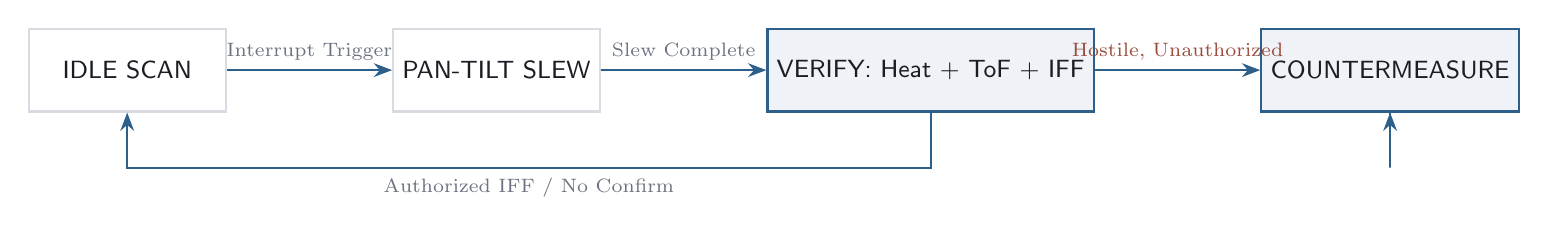
\begin{tikzpicture}[
            node distance=2.1cm,
            state/.style={rectangle, draw=Line, fill=white, thick, minimum height=1.05cm, minimum width=2.5cm, align=center, font=\sffamily\small, text=Ink},
            hoststate/.style={state, draw=Accent, fill=AccentSoft},
            arrow/.style={-Stealth, thick, color=Accent}
        ]
            \node[state] (idle) {IDLE SCAN};
            \node[state, right=of idle] (slew) {PAN-TILT SLEW};
            \node[hoststate, right=of slew] (verify) {VERIFY: Heat + ToF + IFF};
            \node[hoststate, right=of verify] (counter) {COUNTERMEASURE};

            \draw[arrow] (idle) -- node[above, font=\scriptsize, color=Dim]{Interrupt Trigger} (slew);
            \draw[arrow] (slew) -- node[above, font=\scriptsize, color=Dim]{Slew Complete} (verify);
            \draw[arrow] (verify) -- node[above, font=\scriptsize, color=Warn]{Hostile, Unauthorized} (counter);
            \draw[arrow] (verify.south) -- ++(0,-0.7) -| node[near start, below, font=\scriptsize, color=Dim]{Authorized IFF / No Confirm} (idle.south);
            \draw[arrow] (counter.south) -- ++(0,-0.7) -| (idle.south -| counter.south);
        \end{tikzpicture}
    }
    \vspace{0.2cm}
    \small\color{Dim} The ATmega32 acts as the central real-time FSM: signal acquisition, bus arbitration, timing, and peripheral management all run on a single controller.
\end{frame}

% --- SLIDE 10: ROLE OF THE ATMEGA32 - PERIPHERAL UTILIZATION ---
\begin{frame}{4. Role of the ATmega32}{Peripheral Utilization Breakdown}
    \footnotesize
    \begin{itemize}
        \item \textbf{GPIO:} MOSFET power stages, status indicators, SPI chip-select lines.
        \item \textbf{External interrupts (INT0/1/2):} sub-millisecond intrusion detection across 3 sectors, no polling overhead.
        \item \textbf{Timer0 \& Timer2 (8-bit):} Phase-Correct/Fast PWM, 50 Hz on OC0 and OC2 for dual-axis servo positioning.
        \item \textbf{Timer1 (16-bit):} microsecond system clock for non-blocking task scheduling.
        \item \textbf{Hardware TWI (I$^2$C):} 100 kHz bus to MLX90614 (0x5A), VL53L0X (0x29), and local LCD.
        \item \textbf{Hardware SPI:} 4 MHz master mode, multiplexed between nRF24L01+ and MicroSD via software CS.
        \item \textbf{Hardware USART:} 115200 baud, continuous telemetry frames (\texttt{\$ANGLE, DIST, TEMP, STATUS\#}).
        \item \textbf{ADC:} reads supply voltage on ADC0 to detect low-power conditions.
    \end{itemize}
\end{frame}

% --- SLIDE 11: IMPLEMENTATION PLAN - MILESTONES ---
\begin{frame}{5. Implementation Plan}{Milestones}
    \begin{columns}[T]
        \begin{column}{0.48\textwidth}
            \begin{block}{Project Update 1 (Wks 1--3)}
                \footnotesize
                \begin{itemize}
                    \item 1.1 Bare-metal clock, power, register setup
                    \item 1.2 Timer0/Timer2 50 Hz PWM for dual-axis servos
                    \item 1.3 Hardware I$^2$C driver: MLX90614 + VL53L0X
                    \item 1.4 External interrupts for sector detection
                \end{itemize}
                \textbf{Deliverable:} turret slews to activated sector, outputs distance/temperature over UART.
            \end{block}
        \end{column}
        \begin{column}{0.48\textwidth}
            \begin{block}{Final Demonstration (Wks 4--6)}
                \footnotesize
                \begin{itemize}
                    \item 2.1 SPI multiplexing (nRF24L01+ + MicroSD, independent CS)
                    \item 2.2 Wireless IFF challenge-response handshake
                    \item 2.3 Python PC tactical radar GUI over UART
                    \item 2.4 Countermeasure MOSFET drive integration
                    \item 2.5 Enclosure, power decoupling, stress test, tuning
                \end{itemize}
                \textbf{Deliverable:} full platform -- detection, tracking, IFF, radar.
            \end{block}
        \end{column}
    \end{columns}
\end{frame}

% --- SLIDE 12: IMPLEMENTATION PLAN - TEAM RESPONSIBILITIES ---
\begin{frame}{5. Implementation Plan}{Group Member Responsibilities}
    \begin{columns}[T]
        \begin{column}{0.32\textwidth}
            \begin{block}{Member 1: Firmware \& Control}
                \small
                \begin{itemize}
                    \item Register-level drivers (Timers, PWM, I$^2$C, ext.\ interrupts)
                    \item Core FSM architecture
                    \item Timing loop optimization
                \end{itemize}
            \end{block}
        \end{column}
        \begin{column}{0.32\textwidth}
            \begin{block}{Member 2: Hardware, Power \& Actuation}
                \small
                \begin{itemize}
                    \item Pan-tilt turret assembly
                    \item Power distribution / decoupling
                    \item Sensor calibration; MOSFET driver circuitry
                \end{itemize}
            \end{block}
        \end{column}
        \begin{column}{0.32\textwidth}
            \begin{block}{Member 3: Wireless, Storage \& GUI}
                \small
                \begin{itemize}
                    \item SPI bus mgmt.\ (nRF24L01+ + MicroSD)
                    \item IFF protocol logic
                    \item Python tactical radar GUI
                \end{itemize}
            \end{block}
        \end{column}
    \end{columns}
\end{frame}

% --- SLIDE 13: USE OF OTHER CONTROLLERS ---
\begin{frame}{6. Use of Other Controllers}{Optional Auxiliary Node}
    \begin{block}{Main System}
        \small The ATmega32 is the sole main microcontroller: all core logic, sensor readings, motor drives, storage logging, and telemetry streaming run on it.
    \end{block}
    \begin{block}{Auxiliary Controller -- Wearable IFF Badge}
        \small
        \begin{itemize}
            \item \textbf{Device:} Arduino Nano / ATtiny85, battery-powered, worn by personnel.
            \item \textbf{Why required:} the badge is a mobile node distinct from the fixed turret station.
            \item \textbf{Tasks:} listens for a 2.4 GHz challenge packet from the ATmega32 via its own nRF24L01+ module and responds with a pre-shared 32-bit authorization hash.
            \item \textbf{Interface:} wireless RF only -- performs no main system tasks.
        \end{itemize}
    \end{block}
\end{frame}

% --- SLIDE 14: TESTING AND SUCCESS CRITERIA ---
\begin{frame}{7. Testing \& Success Criteria}{Measurable Criteria \& Test Methodology}
    \scriptsize
    \begin{table}
        \centering
        \begin{tabular}{llll}
            \toprule
            \textbf{\color{Accent} Metric} & \textbf{\color{Accent} Target} & \textbf{\color{Accent} Test Method} & \textbf{\color{Accent} Priority} \\
            \midrule
            Turret slew speed & $< 500$ ms & Trigger-to-motion timing & Essential \\
            Distance range \& precision & $\pm 5$ mm at $\le 1.5$ m & VL53L0X bench test & Essential \\
            Thermal verification & $\Delta T \ge 3^\circ$C above ambient & Controlled heat-source test & Essential \\
            IFF handshake execution & $< 30$ ms & RF range/response timing & Essential \\
            PWM \& turret accuracy & Stable 50 Hz on OC0/OC2 & Oscilloscope waveform check & Essential \\
            I$^2$C bus stability & Clean SCL @ 100 kHz & Multi-device signal integrity & Essential \\
            Telemetry streaming rate & $\ge 10$ Hz, no frame loss & PC GUI continuous update & Optional \\
            MicroSD black-box log & Event timestamp/angle/heat & File readback verification & Optional \\
            \bottomrule
        \end{tabular}
    \end{table}
    \vspace{0.2cm}
    \footnotesize\color{Dim} Essential: multi-sector interrupt detection, dual-axis PWM tracking, I$^2$C thermal/ToF check, basic countermeasure trigger. Optional: MicroSD logger, PC radar GUI, audio warning tone, ADC battery monitor.
\end{frame}

% --- SLIDE 15: CHALLENGES AND FUTURE SCOPE ---
\begin{frame}{8. Challenges \& Future Scope}{Anticipated Issues \& Scaling Path}
    \begin{columns}[T]
        \begin{column}{0.48\textwidth}
            \begin{block}{Technical \& Hardware Challenges}
                \footnotesize
                \begin{itemize}
                    \item \textbf{SPI bus contention:} nRF24L01+ (low latency) vs.\ MicroSD (bulk writes) $\rightarrow$ dedicated CS lines, explicit bus-release routines.
                    \item \textbf{Inductive noise:} servo current spikes risk brown-out $\rightarrow$ isolated 5V/6V buck rails, 1000\,$\mu$F decoupling.
                    \item \textbf{Non-blocking I$^2$C:} slow sensor response could stall main loop $\rightarrow$ state-driven polling, no blocking delays.
                \end{itemize}
            \end{block}
        \end{column}
        \begin{column}{0.48\textwidth}
            \begin{block}{Future Scope}
                \footnotesize
                \begin{itemize}
                    \item \textbf{Computer vision:} ESP32-CAM co-processor for facial recognition / visual target classification.
                    \item \textbf{360$^\circ$ slewing:} continuous stepper motors and slip rings for full perimeter coverage.
                    \item \textbf{Long-range telemetry:} LoRa mesh for multi-kilometer, multi-unit perimeter networking.
                \end{itemize}
            \end{block}
        \end{column}
    \end{columns}
\end{frame}

\end{document}
